\documentclass[12pt,a4paper]{article}

\usepackage[margin=1in]{geometry}
\usepackage{amsmath, amssymb, amsthm}
\usepackage{mathtools}
\usepackage{enumitem}
\usepackage{booktabs}
\usepackage{array}
\usepackage{xcolor}
\usepackage{tikz}
\usetikzlibrary{arrows.meta, positioning}

\setlength{\parindent}{0pt}
\setlength{\parskip}{6pt}

\newtheoremstyle{lecturestyle}
  {8pt}
  {8pt}
  {\normalfont}
  {}
  {\bfseries}
  {.}
  {0.5em}
  {}

\theoremstyle{lecturestyle}
\newtheorem{definition}{Definition}
\newtheorem{example}{Example}
\newtheorem{proposition}{Proposition}
\newtheorem{corollary}{Corollary}
\newtheorem{remark}{Remark}

\newenvironment{answer}
{\par\textbf{Answer.}\ }
{\hfill$\square$\par}

\newcommand{\Prob}{\mathbb{P}}
\newcommand{\E}{\mathbb{E}}

\title{\textbf{Lecture 8: Long-Run Behaviour of Markov Chains}}
\author{MA4034: Time Series and Stochastic Processes}
\date{}

\begin{document}
\maketitle

\section{From Immediate Behaviour to Long-Run Behaviour}

In time series analysis, we often study the behaviour of a process over time and try to predict what happens in the near future. For example, if we observe today's value, we may want to predict tomorrow's value.

In stochastic processes, especially Markov chains, we are also interested in a different question:
\[
\text{What happens to the system in the long run?}
\]
That is, instead of only asking for the immediate next step, we ask for the limiting behaviour as time becomes very large.

Mathematically, we study limits such as
\[
\lim_{n\to\infty}p_{ij}^{(n)}
\]
or
\[
\lim_{n\to\infty}P^n.
\]

\textbf{Analogy.} If a person takes one step at a time, the next step tells us where they will be immediately. But if we watch for a long time, we may want to know whether they keep moving around, get trapped somewhere, or settle into a stable pattern. Lecture 8 is about this long-run picture.

\section{Review from Lecture 7}

Let $\{X_n:n=0,1,2,\ldots\}$ be a Markov chain with state space $S$. The Markov property is
\[
\Prob(X_{n+1}=j\mid X_0=i_0,\ldots,X_n=i)
=
\Prob(X_{n+1}=j\mid X_n=i).
\]

For a time-homogeneous Markov chain,
\[
p_{ij}=\Prob(X_{n+1}=j\mid X_n=i)
\]
does not depend on $n$. The value $p_{ij}$ is called the one-step transition probability from state $i$ to state $j$.

The transition probabilities satisfy
\[
p_{ij}\geq 0,
\qquad
\sum_{j\in S}p_{ij}=1
\]
for every state $i$.

When the transition probabilities are collected in a matrix
\[
P=(p_{ij}),
\]
we call $P$ the transition matrix. Matrix notation is useful because it allows us to apply matrix operations and linear algebra to Markov chain calculations.

\begin{remark}
Each row of a transition matrix is a probability distribution over the possible next states. Therefore the row sum must always be 1.
\end{remark}

\section{Time Dynamics of a Markov Chain}

The one-step transition matrix $P$ tells us what can happen after one step. But often we want probabilities after two, three, or many steps.

The $n$-step transition probability is
\[
p_{ij}^{(n)}=\Prob(X_n=j\mid X_0=i).
\]
This is the probability that the chain is in state $j$ after $n$ steps, given that it started in state $i$.

\subsection{Two-Step Transitions}

Suppose the chain starts in state $i$ at time $t=n$ and is in state $j$ at time $t=n+2$. To move from $i$ to $j$ in two steps, the chain must pass through some intermediate state $k$ at time $t=n+1$.

Therefore,
\[
p_{ij}^{(2)}=\sum_{k\in S}p_{ik}p_{kj}.
\]

\begin{center}
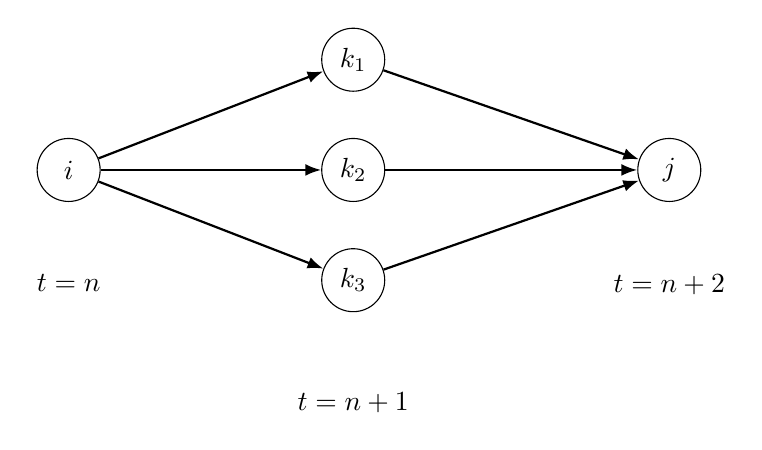
\begin{tikzpicture}[
  state/.style={circle, draw, minimum size=8mm},
  edge/.style={-{Latex[length=2mm]}, thick},
  node distance=24mm
]
\node[state] (i) {$i$};
\node[state, right=28mm of i, yshift=14mm] (k1) {$k_1$};
\node[state, right=28mm of i] (k2) {$k_2$};
\node[state, right=28mm of i, yshift=-14mm] (k3) {$k_3$};
\node[state, right=32mm of k2] (j) {$j$};

\draw[edge] (i) -- (k1);
\draw[edge] (i) -- (k2);
\draw[edge] (i) -- (k3);
\draw[edge] (k1) -- (j);
\draw[edge] (k2) -- (j);
\draw[edge] (k3) -- (j);

\node[below=8mm of i] {$t=n$};
\node[below=23mm of k2] {$t=n+1$};
\node[below=8mm of j] {$t=n+2$};
\end{tikzpicture}
\end{center}

Each possible intermediate state contributes one term to the summation.

\subsection{Three-Step and Multi-Step Transitions}

If there are two intermediate states, say $k_1$ and $k_2$, then
\[
p_{ij}^{(3)}
=
\sum_{k_1\in S}\sum_{k_2\in S}
p_{ik_1}p_{k_1k_2}p_{k_2j}.
\]

For each intermediate time point, we need another summation. This can become costly and time-consuming if we do the calculations manually.

\section{Chapman--Kolmogorov Equations}

To simplify multi-step calculations, we use the Chapman--Kolmogorov equations.

\begin{proposition}[Chapman--Kolmogorov Equations]
For a time-homogeneous Markov chain,
\[
p_{ij}^{(n+m)}
=
\sum_{k\in S}p_{ik}^{(n)}p_{kj}^{(m)}.
\]
In matrix form,
\[
P^{(n+m)}=P^{(n)}P^{(m)}.
\]
\end{proposition}

Since $P^{(1)}=P$, it follows that
\[
P^{(n)}=P^n.
\]
Therefore, to find the $n$-step transition probability from state $i$ to state $j$:
\[
\boxed{p_{ij}^{(n)}=\text{the }(i,j)\text{ entry of }P^n.}
\]

\textbf{Analogy.} Matrix multiplication works like adding up all possible routes. If there are many paths from $i$ to $j$, the matrix product automatically multiplies probabilities along each path and then adds over all possible paths.

\section{Limiting Transition Probabilities}

To understand long-run behaviour, we study
\[
\lim_{n\to\infty}P^n.
\]
If this limit exists, it describes the final or long-run probabilities of the system.

\subsection{Genetics Example}

Recall the genetics transition matrix with state order
\[
S=\{AA,Aa,aa\}:
\]
\[
P=
\begin{pmatrix}
1 & 0 & 0\\
\frac14 & \frac12 & \frac14\\
0 & 0 & 1
\end{pmatrix}.
\]

The limiting transition matrix is
\[
\lim_{n\to\infty}P^n
=
\begin{pmatrix}
1 & 0 & 0\\
\frac12 & 0 & \frac12\\
0 & 0 & 1
\end{pmatrix}.
\]

This says:
\begin{itemize}[leftmargin=1.2cm]
    \item If the chain starts at $AA$, it remains at $AA$ forever.
    \item If the chain starts at $Aa$, it eventually moves to either $AA$ or $aa$.
    \item If the chain starts at $aa$, it remains at $aa$ forever.
\end{itemize}

The exact immediate result may not be predictable, but the limiting result can often be described.

\section{Example: ON/OFF System}

Consider a system with two states:
\[
0=\text{OFF}, \qquad 1=\text{ON}.
\]
At each discrete time point:
\begin{itemize}[leftmargin=1.2cm]
    \item If the system is OFF, it switches to ON with probability $p$.
    \item If the system is ON, it switches to OFF with probability $q$.
\end{itemize}

The transition diagram is:

\begin{center}
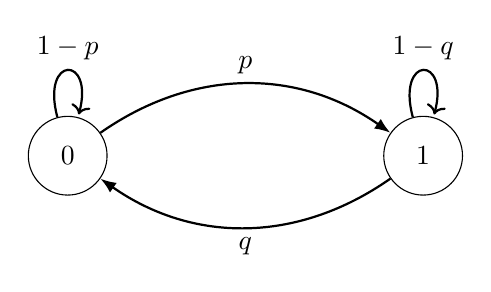
\begin{tikzpicture}[
  state/.style={circle, draw, minimum size=10mm},
  edge/.style={-{Latex[length=2mm]}, thick},
  bend angle=35
]
\node[state] (0) {$0$};
\node[state, right=35mm of 0] (1) {$1$};

\draw[edge] (0) edge[loop above] node {$1-p$} (0);
\draw[edge] (1) edge[loop above] node {$1-q$} (1);
\draw[edge] (0) edge[bend left] node[above] {$p$} (1);
\draw[edge] (1) edge[bend left] node[below] {$q$} (0);
\end{tikzpicture}
\end{center}

Using the state order $\{0,1\}$, the transition matrix is
\[
P=
\begin{pmatrix}
1-p & p\\
q & 1-q
\end{pmatrix}.
\]

\subsection{Finding the $n$-Step Transition Matrix}

To calculate $P^n$, we may use eigenvalues and eigenvectors. For the ON/OFF system, the eigenvalues are
\[
\lambda_1=1,
\qquad
\lambda_2=1-p-q.
\]

When $p+q\neq 0$, the $n$-step transition matrix is
\[
P^n
=
\frac{1}{p+q}
\begin{pmatrix}
q & p\\
q & p
\end{pmatrix}
+
\frac{(1-p-q)^n}{p+q}
\begin{pmatrix}
p & -p\\
-q & q
\end{pmatrix}.
\]

If $|1-p-q|<1$, then
\[
\lim_{n\to\infty}(1-p-q)^n=0.
\]
Thus,
\[
\lim_{n\to\infty}P^n
=
\frac{1}{p+q}
\begin{pmatrix}
q & p\\
q & p
\end{pmatrix}.
\]

This means that, in the long run,
\[
\Prob(\text{OFF})=\frac{q}{p+q},
\qquad
\Prob(\text{ON})=\frac{p}{p+q}.
\]

\textbf{Interpretation.} If $q>p$, the system switches from ON to OFF more easily than it switches from OFF to ON. Therefore the long-run probability of being OFF is larger.

\begin{example}[ON/OFF System Calculation]
Suppose $p=\frac34$ and $q=\frac12$. If the system starts OFF, find the probability that it is ON at time $n=3$.
\end{example}

\begin{answer}
We need the $(0,1)$ entry of $P^3$.

Here,
\[
p+q=\frac34+\frac12=\frac54
\]
and
\[
\lambda_2=1-p-q
=1-\frac34-\frac12
=-\frac14.
\]

The $(0,1)$ entry of $P^n$ is
\[
p_{01}^{(n)}
=
\frac{p}{p+q}
 \frac{(1-p-q)^n}{p+q}(-p).
\]
Therefore,
\[
p_{01}^{(n)}
=
\frac{p}{p+q}\left[1-(1-p-q)^n\right].
\]
For $n=3$,
\[
p_{01}^{(3)}
=
\frac{3/4}{5/4}
\left(\frac{-3/4}{5/4}\right)\left(-\frac14\right)^3.
\]
So,
\[
p_{01}^{(3)}
=
\frac35+\left(-\frac35\right)\left(-\frac{1}{64}\right)
=
\frac35+\frac{3}{320}
=
\frac{195}{320}
=
\frac{39}{64}.
\]
Thus the probability that the system is ON at time 3 is
\[
\boxed{\frac{39}{64}\approx 0.6094.}
\]
\end{answer}

\section{Eigenvalue Refresher}

For a square matrix $P$, an eigenvalue $\lambda$ and eigenvector $v$ satisfy
\[
Pv=\lambda v.
\]

If $P$ can be diagonalized, then
\[
P=RDR^{-1},
\]
where $D$ is a diagonal matrix containing the eigenvalues, and $R$ is a matrix built from the corresponding eigenvectors.

Then
\[
P^n=RD^nR^{-1}.
\]
This is useful because powers of a diagonal matrix are easy:
\[
D^n=
\begin{pmatrix}
\lambda_1^n & 0 & \cdots\\
0 & \lambda_2^n & \cdots\\
\vdots & \vdots & \ddots
\end{pmatrix}.
\]

\textbf{Analogy.} Diagonalization changes coordinates so that the Markov chain separates into simpler independent directions. Raising the matrix to a power then becomes much easier.

\begin{remark}
Even for a $2\times 2$ matrix, calculating $P^n$ directly can be tedious. Eigenvalues and eigenvectors provide a systematic method.
\end{remark}

\section{Classifying States}

To understand limiting behaviour, we need to classify the states of a Markov chain.

\subsection{Accessible States}

\begin{definition}[Accessible]
State $j$ is said to be \textbf{accessible} from state $i$, written
\[
i\to j,
\]
if there exists some $n\geq 0$ such that
\[
p_{ij}^{(n)}>0.
\]
\end{definition}

This means there is a path from $i$ to $j$ with positive probability.

\textbf{Analogy.} If states are towns and arrows are roads, then $j$ is accessible from $i$ if there is a route from town $i$ to town $j$.

\subsection{Communicating States}

\begin{definition}[Communicate]
States $i$ and $j$ are said to \textbf{communicate}, written
\[
i\leftrightarrow j,
\]
if
\[
i\to j
\quad\text{and}\quad
j\to i.
\]
\end{definition}

Communicating states have a two-way connection.

\subsection{Equivalence Classes}

The relation ``communicates with'' groups states into equivalence classes. States in the same class can reach each other.

\begin{example}
In the roulette chain with absorbing state $0$, from state $1$ we can reach state $0$, but from state $0$ we cannot reach state $1$. Thus $0$ is accessible from $1$, but $1$ is not accessible from $0$.

The states $1,2,3,\ldots$ communicate with each other because it is possible to move up or down among positive states.
\end{example}

\begin{example}
In the genetics chain, $AA$ and $aa$ are absorbing states. From $Aa$, the chain can reach $AA$ or $aa$, but once it reaches $AA$ or $aa$, it cannot return to $Aa$. Thus the communication classes are
\[
\{AA\},\qquad \{Aa\},\qquad \{aa\}.
\]
\end{example}

\begin{example}
In the ON/OFF chain with $p>0$ and $q>0$, state $0$ can reach state $1$ and state $1$ can reach state $0$. Therefore the states communicate:
\[
0\leftrightarrow 1.
\]
\end{example}

\subsection{Irreducibility}

\begin{definition}[Irreducible Markov Chain]
A Markov chain is called \textbf{irreducible} if all states communicate with each other.
\end{definition}

In an irreducible chain, the whole state space forms one communicating class.

\section{Recurrent and Transient States}

Let $i$ be a state. Define the first return time to state $i$ as
\[
\tau_i=\min\{n\geq 1:X_n=i\}.
\]
If the chain never returns to $i$, we set
\[
\tau_i=\infty.
\]

\begin{definition}[Recurrent State]
A state $i$ is called \textbf{recurrent} if
\[
\Prob_i(\tau_i<\infty)=1.
\]
That is, starting from state $i$, the chain returns to $i$ eventually with probability 1.
\end{definition}

\begin{definition}[Transient State]
A state $i$ is called \textbf{transient} if
\[
\Prob_i(\tau_i<\infty)<1.
\]
That is, starting from state $i$, there is a positive probability that the chain never returns to $i$.
\end{definition}

The idea is simple:
\[
\begin{array}{c|c|c}
\text{Condition} & \text{Meaning} & \text{Classification}\\
\hline
\Prob_i(\tau_i<\infty)=1 & \text{we return to }i\text{ sometime} & \text{recurrent}\\
\Prob_i(\tau_i<\infty)<1 & \text{we may never return to }i & \text{transient}
\end{array}
\]

\textbf{Analogy.} A recurrent state is like a home that you are guaranteed to revisit eventually. A transient state is like a place you may pass through and then possibly never see again.

\subsection{Examples}

In the roulette chain with absorbing state $0$:
\begin{itemize}[leftmargin=1.2cm]
    \item State $0$ is recurrent because once the chain reaches $0$, it stays there.
    \item Positive states may be transient because the chain may reach $0$ and then never return to them.
\end{itemize}

In the genetics chain:
\begin{itemize}[leftmargin=1.2cm]
    \item $AA$ and $aa$ are recurrent absorbing states.
    \item $Aa$ is transient because once the chain leaves $Aa$ and reaches $AA$ or $aa$, it cannot return.
\end{itemize}

In the ON/OFF chain with $p>0$ and $q>0$:
\begin{itemize}[leftmargin=1.2cm]
    \item Both states are recurrent.
    \item The states communicate with each other.
\end{itemize}

\begin{corollary}
In an irreducible Markov chain, either all states are recurrent or all states are transient.
\end{corollary}

\begin{corollary}
Suppose the state space is finite. A state $i$ is transient if and only if there is another state $j$ such that
\[
i\to j
\quad\text{but}\quad
j\nrightarrow i.
\]
\end{corollary}

\section{Absorbing States}

\begin{definition}[Absorbing State]
A state $i$ is absorbing if
\[
p_{ii}=1.
\]
Once the chain enters an absorbing state, it can never leave.
\end{definition}

In the roulette example, state $0$ is absorbing. If the player reaches \$0, the player is ruined and cannot continue. Hence
\[
p_{00}=1.
\]

\section{A Series Criterion for Recurrence}

Let
\[
I_n=
\begin{cases}
1, & X_n=i,\\
0, & X_n\neq i.
\end{cases}
\]
Then
\[
S=\sum_{n=1}^{\infty}I_n
\]
counts the total number of returns to state $i$.

Taking expectation when starting from $i$,
\[
\E_i[S]
=
\sum_{n=1}^{\infty}\E_i[I_n]
=
\sum_{n=1}^{\infty}\Prob_i(X_n=i)
=
\sum_{n=1}^{\infty}p_{ii}^{(n)}.
\]

\begin{proposition}[Recurrence Criterion]
State $i$ is transient if
\[
\sum_{n=1}^{\infty}p_{ii}^{(n)}<\infty.
\]
State $i$ is recurrent if
\[
\sum_{n=1}^{\infty}p_{ii}^{(n)}=\infty.
\]
\end{proposition}

This proposition is not always the easiest tool to apply, but it is important because it connects recurrence with the long-run behaviour of the powers of the transition matrix.

\section{Stationary Distributions}

\begin{definition}[Stationary Distribution]
A probability row vector
\[
\pi=(\pi_0,\pi_1,\pi_2,\ldots)
\]
is called a \textbf{stationary distribution} for a Markov chain with transition matrix $P$ if
\[
\pi P=\pi
\]
and
\[
\pi_i\geq 0,\qquad \sum_{i\in S}\pi_i=1.
\]
\end{definition}

The equation $\pi P=\pi$ means that if the chain starts with distribution $\pi$, then after one transition it still has distribution $\pi$. The distribution is unchanged by the transition matrix.

\textbf{Analogy.} A stationary distribution is like a perfectly balanced traffic pattern. Cars may continue moving between towns, but the proportion of cars in each town remains the same after each time step.

\subsection{How to Find a Stationary Distribution}

To find $\pi$, solve
\[
\pi P=\pi
\]
together with
\[
\sum_{i\in S}\pi_i=1.
\]

Equivalently,
\[
\pi(P-I)=0
\]
or
\[
\pi(I-P)=0,
\]
depending on how the equation is rearranged.

The zero vector is always a solution of the homogeneous linear system, but it is not a probability distribution. Therefore we must also impose
\[
\sum_{i\in S}\pi_i=1
\]
and
\[
\pi_i\geq 0.
\]

\begin{proposition}
For an irreducible Markov chain, if a stationary distribution exists, then it is unique.
\end{proposition}

\begin{proposition}
If the state space $S$ is finite and the Markov chain is irreducible, then a unique stationary distribution exists.
\end{proposition}

\section{Stationary Distribution Examples}

\begin{example}[Stationary Distributions for the Genetics Chain]
For
\[
P=
\begin{pmatrix}
1 & 0 & 0\\
\frac14 & \frac12 & \frac14\\
0 & 0 & 1
\end{pmatrix},
\]
find the stationary distributions.
\end{example}

\begin{answer}
Let
\[
\pi=(\pi_{AA},\pi_{Aa},\pi_{aa}).
\]
We solve
\[
\pi P=\pi.
\]
That is,
\[
(\pi_{AA},\pi_{Aa},\pi_{aa})
\begin{pmatrix}
1 & 0 & 0\\
\frac14 & \frac12 & \frac14\\
0 & 0 & 1
\end{pmatrix}
=
(\pi_{AA},\pi_{Aa},\pi_{aa}).
\]

This gives
\[
\pi_{AA}+\frac14\pi_{Aa}=\pi_{AA},
\]
\[
\frac12\pi_{Aa}=\pi_{Aa},
\]
\[
\frac14\pi_{Aa}+\pi_{aa}=\pi_{aa}.
\]

From the first equation,
\[
\frac14\pi_{Aa}=0,
\]
so
\[
\pi_{Aa}=0.
\]
The remaining probability must be split between $AA$ and $aa$:
\[
\pi_{AA}+\pi_{aa}=1.
\]
Therefore every distribution of the form
\[
\boxed{\pi=(\alpha,0,1-\alpha),\qquad 0\leq \alpha\leq 1}
\]
is stationary.

There is not a unique stationary distribution because the chain is not irreducible.
\end{answer}

\begin{example}[Stationary Distribution of the ON/OFF Chain]
Find the stationary distribution of
\[
P=
\begin{pmatrix}
1-p & p\\
q & 1-q
\end{pmatrix}
\]
where $p,q>0$.
\end{example}

\begin{answer}
Let
\[
\pi=(\pi_0,\pi_1).
\]
We solve
\[
\pi P=\pi
\]
and
\[
\pi_0+\pi_1=1.
\]

The first component gives
\[
(1-p)\pi_0+q\pi_1=\pi_0.
\]
Rearranging,
\[
-p\pi_0+q\pi_1=0,
\]
so
\[
q\pi_1=p\pi_0.
\]
Thus,
\[
\pi_1=\frac{p}{q}\pi_0.
\]

Using $\pi_0+\pi_1=1$,
\[
\pi_0+\frac{p}{q}\pi_0=1.
\]
Therefore,
\[
\pi_0\left(\frac{p+q}{q}\right)=1,
\]
so
\[
\pi_0=\frac{q}{p+q}.
\]
Then
\[
\pi_1=\frac{p}{p+q}.
\]

Hence the stationary distribution is
\[
\boxed{\pi=\left(\frac{q}{p+q},\frac{p}{p+q}\right).}
\]
\end{answer}

\section{Infinite-State Example and Non-Existence}

Consider the fair gambler's chain on
\[
S=\{0,1,2,\ldots\}
\]
with transition matrix
\[
P=
\begin{pmatrix}
\frac12 & \frac12 & 0 & 0 & \cdots\\
\frac12 & 0 & \frac12 & 0 & \cdots\\
0 & \frac12 & 0 & \frac12 & \cdots\\
\vdots & \vdots & \vdots & \vdots & \ddots
\end{pmatrix}.
\]

This chain is recurrent, but it does not have a stationary distribution.

To see why, let
\[
\pi=(\pi_0,\pi_1,\pi_2,\ldots).
\]
From $\pi P=\pi$, the equations imply
\[
\pi_0=\pi_1=\pi_2=\cdots.
\]
So all probabilities must be equal.

If the common value is 0, then
\[
\sum_{i=0}^{\infty}\pi_i=0,
\]
which is not 1. If the common value is positive, then
\[
\sum_{i=0}^{\infty}\pi_i=\infty.
\]
Therefore no probability distribution $\pi$ can satisfy the equations.

Hence no stationary distribution exists.

\section{What if the Winning Probability is Less Than $\frac12$?}

Now consider a biased chain on
\[
S=\{0,1,2,\ldots\}
\]
where the probability of moving up is $p$ and the probability of moving down is $1-p$, with
\[
p<\frac12.
\]

The transition matrix is
\[
P=
\begin{pmatrix}
1-p & p & 0 & 0 & \cdots\\
1-p & 0 & p & 0 & \cdots\\
0 & 1-p & 0 & p & \cdots\\
\vdots & \vdots & \vdots & \vdots & \ddots
\end{pmatrix}.
\]

Solving $\pi P=\pi$ gives
\[
\pi_n=
\left(\frac{p}{1-p}\right)^n\pi_0,
\qquad n=0,1,2,\ldots
\]

Since $p<1/2$,
\[
\frac{p}{1-p}<1.
\]
Therefore the geometric series converges:
\[
1
=
\sum_{n=0}^{\infty}\pi_n
=
\pi_0\sum_{n=0}^{\infty}\left(\frac{p}{1-p}\right)^n.
\]
Using
\[
\sum_{n=0}^{\infty}r^n=\frac{1}{1-r}, \qquad |r|<1,
\]
with
\[
r=\frac{p}{1-p},
\]
we get
\[
1
=
\pi_0\frac{1}{1-\frac{p}{1-p}}
=
\pi_0\frac{1-p}{1-2p}.
\]
Thus
\[
\pi_0=\frac{1-2p}{1-p}.
\]

Therefore,
\[
\boxed{
\pi_n=
\frac{1-2p}{1-p}
\left(\frac{p}{1-p}\right)^n,
\qquad n=0,1,2,\ldots
}
\]
is the stationary distribution.

The key reason this works is that the geometric series converges when $p<1/2$.

\section{Positive Recurrent and Null Recurrent States}

\begin{definition}[Positive Recurrent State]
Let $i$ be a recurrent state. If
\[
\E_i[\tau_i]<\infty,
\]
then $i$ is called \textbf{positive recurrent}.
\end{definition}

\begin{definition}[Null Recurrent State]
Let $i$ be a recurrent state. If
\[
\E_i[\tau_i]=\infty,
\]
then $i$ is called \textbf{null recurrent}.
\end{definition}

So recurrence only says that the chain returns eventually with probability 1. Positive recurrence says that the expected return time is finite. Null recurrence says that the chain returns eventually, but the expected return time is infinite.

\begin{corollary}
For an irreducible Markov chain, there are three possibilities:
\begin{itemize}[leftmargin=1.2cm]
    \item all states are positive recurrent,
    \item all states are null recurrent,
    \item all states are transient.
\end{itemize}
\end{corollary}

\begin{proposition}
For an irreducible Markov chain, a stationary distribution exists if and only if the chain is positive recurrent. In this case, the stationary distribution is unique and satisfies
\[
\pi_i>0
\]
for all states $i$.
\end{proposition}

Therefore, two important conditions for a unique stationary distribution are:
\[
\boxed{\text{irreducible and positive recurrent}.}
\]

\section{Worked Examples}

\begin{example}[Computing a Two-Step Probability]
Let
\[
P=
\begin{pmatrix}
0.7 & 0.3\\
0.4 & 0.6
\end{pmatrix}.
\]
Find $p_{01}^{(2)}$.
\end{example}

\begin{answer}
Using
\[
p_{01}^{(2)}=\sum_{k\in S}p_{0k}p_{k1},
\]
we get
\[
p_{01}^{(2)}
=p_{00}p_{01}+p_{01}p_{11}.
\]
Substitute the values:
\[
p_{01}^{(2)}
=(0.7)(0.3)+(0.3)(0.6).
\]
Thus,
\[
p_{01}^{(2)}
=0.21+0.18
=0.39.
\]
\end{answer}

\begin{example}[Classifying States]
Consider a Markov chain with states $\{0,1,2\}$ and transition diagram:
\[
0\to 1,\qquad 1\to 2,\qquad 2\to 2.
\]
Classify the states as transient or recurrent.
\end{example}

\begin{answer}
State $2$ is absorbing because once the chain reaches $2$, it stays at $2$. Hence state $2$ is recurrent.

State $0$ can move to $1$, then to $2$, but it cannot return to $0$. Therefore state $0$ is transient.

State $1$ can move to $2$, but cannot return to $1$. Therefore state $1$ is transient.
\end{answer}

\begin{example}[Finding a Stationary Distribution]
Find the stationary distribution of
\[
P=
\begin{pmatrix}
0.8 & 0.2\\
0.3 & 0.7
\end{pmatrix}.
\]
\end{example}

\begin{answer}
Let
\[
\pi=(\pi_0,\pi_1).
\]
Solve
\[
\pi P=\pi,
\qquad
\pi_0+\pi_1=1.
\]

From the first component,
\[
0.8\pi_0+0.3\pi_1=\pi_0.
\]
Rearrange:
\[
0.3\pi_1=0.2\pi_0.
\]
Thus,
\[
\pi_1=\frac{2}{3}\pi_0.
\]
Using the sum condition,
\[
\pi_0+\frac23\pi_0=1.
\]
Therefore,
\[
\frac53\pi_0=1,
\]
so
\[
\pi_0=\frac35.
\]
Then
\[
\pi_1=\frac25.
\]
Thus,
\[
\boxed{\pi=\left(\frac35,\frac25\right).}
\]
\end{answer}

\section{Summary}

\begin{itemize}[leftmargin=1.2cm]
    \item The $n$-step transition probability is $p_{ij}^{(n)}=\Prob(X_n=j\mid X_0=i)$.
    \item The $n$-step transition matrix is $P^n$.
    \item The Chapman--Kolmogorov equations are
    \[
    p_{ij}^{(n+m)}=\sum_{k\in S}p_{ik}^{(n)}p_{kj}^{(m)}.
    \]
    \item Long-run behaviour is studied using $\lim_{n\to\infty}P^n$.
    \item State $j$ is accessible from state $i$ if $i\to j$.
    \item States $i$ and $j$ communicate if $i\to j$ and $j\to i$.
    \item A chain is irreducible if all states communicate with each other.
    \item A recurrent state is revisited eventually with probability 1.
    \item A transient state may never be revisited.
    \item A stationary distribution satisfies $\pi P=\pi$, $\pi_i\geq 0$, and $\sum_i\pi_i=1$.
    \item For irreducible chains, a stationary distribution exists exactly when the chain is positive recurrent.
\end{itemize}

\section{Essay-Type Questions}

\begin{enumerate}[label=\textbf{Q\arabic*.}, leftmargin=1.2cm]
    \item Explain the meaning of $n$-step transition probabilities. Derive the two-step transition formula using the law of total probability.
    \item State and explain the Chapman--Kolmogorov equations. Why are they useful in Markov chain calculations?
    \item For the ON/OFF system, construct the transition matrix and derive the limiting distribution.
    \item Define accessible states, communicating states, equivalence classes, and irreducibility. Explain these ideas using examples.
    \item Define recurrent and transient states. Classify the states in the genetics example and the roulette example.
    \item Define a stationary distribution. Explain how to find it and why the additional conditions $\pi_i\geq0$ and $\sum_i\pi_i=1$ are necessary.
    \item Explain the difference between positive recurrent and null recurrent states. State the relationship between positive recurrence and stationary distributions.
\end{enumerate}

\section{Answers to Essay-Type Questions}

\subsection*{Answer 1}

The $n$-step transition probability is
\[
p_{ij}^{(n)}=\Prob(X_n=j\mid X_0=i).
\]
It gives the probability that a Markov chain starting from state $i$ will be in state $j$ after $n$ steps.

For two steps, suppose the chain starts at $i$ and ends at $j$. It must pass through some intermediate state $k$ after one step. Therefore, by the law of total probability,
\[
p_{ij}^{(2)}
=
\sum_{k\in S}\Prob(X_2=j,X_1=k\mid X_0=i).
\]
Using the multiplication rule,
\[
p_{ij}^{(2)}
=
\sum_{k\in S}
\Prob(X_2=j\mid X_1=k,X_0=i)\Prob(X_1=k\mid X_0=i).
\]
By the Markov property,
\[
\Prob(X_2=j\mid X_1=k,X_0=i)
=
\Prob(X_2=j\mid X_1=k)
=p_{kj}.
\]
Also,
\[
\Prob(X_1=k\mid X_0=i)=p_{ik}.
\]
Hence
\[
p_{ij}^{(2)}=\sum_{k\in S}p_{ik}p_{kj}.
\]

\subsection*{Answer 2}

The Chapman--Kolmogorov equations state that
\[
p_{ij}^{(n+m)}
=
\sum_{k\in S}p_{ik}^{(n)}p_{kj}^{(m)}.
\]
This means that to go from $i$ to $j$ in $n+m$ steps, the chain can first go from $i$ to some intermediate state $k$ in $n$ steps, and then from $k$ to $j$ in $m$ more steps.

In matrix form,
\[
P^{(n+m)}=P^{(n)}P^{(m)}.
\]
Since $P^{(1)}=P$, this gives
\[
P^{(n)}=P^n.
\]
The equations are useful because they allow us to compute multi-step transition probabilities by matrix multiplication instead of writing many nested summations.

\subsection*{Answer 3}

The ON/OFF system has states
\[
0=\text{OFF},\qquad 1=\text{ON}.
\]
If the system is OFF, it switches to ON with probability $p$ and remains OFF with probability $1-p$. If it is ON, it switches to OFF with probability $q$ and remains ON with probability $1-q$.

Therefore,
\[
P=
\begin{pmatrix}
1-p & p\\
q & 1-q
\end{pmatrix}.
\]

The stationary distribution $\pi=(\pi_0,\pi_1)$ satisfies
\[
\pi P=\pi,
\qquad
\pi_0+\pi_1=1.
\]
From the first equation,
\[
(1-p)\pi_0+q\pi_1=\pi_0.
\]
Hence
\[
q\pi_1=p\pi_0.
\]
So
\[
\pi_1=\frac{p}{q}\pi_0.
\]
Using $\pi_0+\pi_1=1$,
\[
\pi_0+\frac{p}{q}\pi_0=1.
\]
Thus
\[
\pi_0=\frac{q}{p+q}
\]
and
\[
\pi_1=\frac{p}{p+q}.
\]

Therefore the limiting distribution is
\[
\boxed{\left(\frac{q}{p+q},\frac{p}{p+q}\right)}
\]
when the usual convergence condition $|1-p-q|<1$ holds.

\subsection*{Answer 4}

State $j$ is accessible from state $i$, written $i\to j$, if there is a positive-probability path from $i$ to $j$ in some number of steps:
\[
p_{ij}^{(n)}>0
\]
for some $n\geq0$.

States $i$ and $j$ communicate, written $i\leftrightarrow j$, if
\[
i\to j
\quad\text{and}\quad
j\to i.
\]
Thus communication is a two-way connection.

Communicating states form equivalence classes. These are groups of states that can reach each other.

A Markov chain is irreducible if all states communicate with each other. In other words, the whole state space is one communicating class.

For example, in the ON/OFF chain with $p,q>0$, OFF can reach ON and ON can reach OFF. Therefore the chain is irreducible. In the genetics chain, $AA$ and $aa$ are absorbing, and $Aa$ cannot be reached again once the chain leaves it. Thus the genetics chain is not irreducible.

\subsection*{Answer 5}

Let
\[
\tau_i=\min\{n\geq1:X_n=i\}
\]
be the first return time to state $i$.

State $i$ is recurrent if
\[
\Prob_i(\tau_i<\infty)=1.
\]
This means that, starting from $i$, the chain returns to $i$ eventually with probability 1.

State $i$ is transient if
\[
\Prob_i(\tau_i<\infty)<1.
\]
This means there is a positive probability that the chain never returns to $i$.

In the genetics example, $AA$ and $aa$ are absorbing states, so they are recurrent. State $Aa$ is transient because from $Aa$ the chain may move to $AA$ or $aa$, and after that it cannot return to $Aa$.

In the roulette example with state $0$ absorbing, state $0$ is recurrent. Positive states can be transient because the chain may eventually reach $0$, and once it reaches $0$, it can never return to positive states.

\subsection*{Answer 6}

A stationary distribution is a probability vector $\pi$ satisfying
\[
\pi P=\pi.
\]
It must also satisfy
\[
\pi_i\geq0
\]
and
\[
\sum_{i\in S}\pi_i=1.
\]

To find a stationary distribution, we solve the linear system
\[
\pi P=\pi
\]
together with the probability condition
\[
\sum_i\pi_i=1.
\]

The non-negativity condition is necessary because probabilities cannot be negative. The sum condition is necessary because the total probability over the whole state space must be 1.

The equation $\pi P=\pi$ alone is not enough because it is a homogeneous linear system and may have non-probability solutions, including the zero vector.

\subsection*{Answer 7}

A recurrent state is positive recurrent if the expected return time is finite:
\[
\E_i[\tau_i]<\infty.
\]
It is null recurrent if the expected return time is infinite:
\[
\E_i[\tau_i]=\infty.
\]

Both positive recurrent and null recurrent states are revisited eventually with probability 1. The difference is the average time taken to return. Positive recurrence means the average return time is finite, while null recurrence means the return is guaranteed but may take infinitely long on average.

For an irreducible Markov chain, a stationary distribution exists if and only if the chain is positive recurrent. When it exists, it is unique and has positive probability for every state.

Therefore, for a unique stationary distribution in an irreducible chain, the important condition is positive recurrence.

\end{document}
